\documentclass{article}

\usepackage[utf8]{inputenc}
\usepackage{float}
\usepackage{booktabs}
\usepackage{titling}
\usepackage{listings}
\usepackage{graphicx}
\usepackage{caption}
\usepackage{subcaption}
\usepackage[margin=0.5in]{geometry}
\usepackage{hyperref}



\title{Predicting Runs}
\author{Derek Owens-Oas, Fan Bu, Federico Ferrari, Megan Robertson}
\date{September 24, 2017}

\begin{document}

\maketitle

\section{Introduction}

We chose to investigate the fourth prompt during the NBA Hackathon - create a model to predict exciting runs during games. 

\section{Defining an "exciting" run}

In order to make the project approachable during a 24-hour time period, a simplified definition of run was used to classify every possession in the 2016-2017 season. The algorithm below was used to create the labels for the possession log data. 

\begin{figure}[h]
\begin{center}
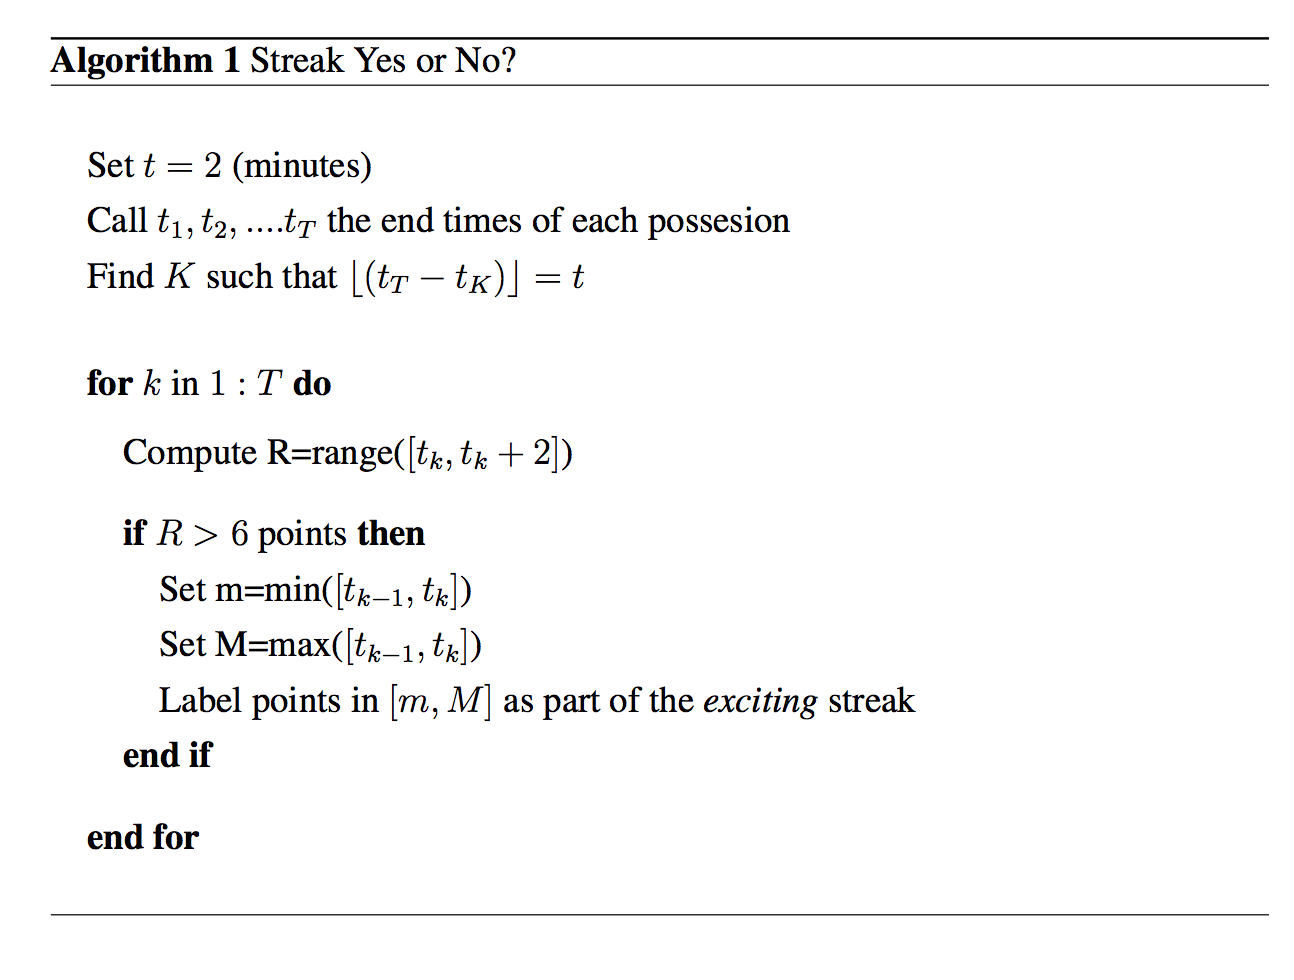
\includegraphics[width=100mm]{run_alg.png}
\caption{Algorithm for Defining Run}
\end{center}
\end{figure}

PLAINER ENGLISH FOR THE NON-STATISTICIANS (THE LAMESIANS, GET IT, NOT BAYESIAN!!!)

- percentage of possessions that are part of a run and those that are not?

\section{Feature Generation}

Multiple variables were added to the possession log data that we thought might be indicative of whether a run was occurring at a certain possession in the game.  Two components that define a run are the pace of the game as well as the points being scored. Typically runs are the result of many rapid plays. Therefore, variables were added for the number of shots taken during a possession as well as the number of rebounds. More shots and more rebounds would be indicative of a team getting many offensive boards and having to work for their basket. The type of shot is also very important to consider when exploring runs. Discussions with our coach and other league mentors led us to add an indicator variable defining whether a shot was a "good" shot. This was arbitrarily defined as any shot that was within six feet of the hoop. This is roughly the areas in and around the key closest to the hoop. \newline

In addition to capturing the variability of runs through the above variables, we also wanted to capture the skill level of the players on the court at the time of the run. Using the play by play data, it was possible to determine the players on the court at the time of each possession. From this, we were able to use external data \footnote{"NBA All Star", \url{http://www.nba-allstar.com/players/lists/players-by-draft-pick.html, 9/23/17}} to determine the number of all stars on the court at the time. This is a very basic way to evaluate skill, but other methods could be used to define quality players. However, given the brief work period we only incorporated the all-star information for the time being. 

\section{Modeling}

We approached predicting exciting runs as a classification problem, each possession in a game can either be classified as being part of a run or not. 

- chart with models

\section{Results}

\end{document}